% This is a sample LaTeX input file.  (Version of 9 April 1986) 
% 
% A '%' character causes TeX to ignore all remaining text on the line, 
% and is used for comments like this one. 

\documentclass[fleqn]{article}    % Specifies the document style. 

\usepackage{graphicx}
\usepackage{psfrag}

%-------------------------
% begin and end equations
%-------------------------
\newcommand{\be} {\begin{equation}}
\newcommand{\ee} {\end{equation}}
\newcommand{\bea}{\begin{eqnarray}}
\newcommand{\eea}{\end{eqnarray}}
\newcommand{\ba} {\begin{array}}
\newcommand{\ea} {\end{array}}

%-----------------
% text formatting 
%-----------------
\newcommand{\noi}{\noindent}

%---------------
% special signs
%---------------
\newcommand{\p}  {\partial}
\newcommand{\s}  {\star}
\newcommand{\Dx} {\Delta}

%-----------------
% velocity vector
%-----------------
\newcommand{\uvw}{{\bf u}}          

%---------------------------
% putting things up or down
%---------------------------
\newcommand{\ol} {\overline}
\newcommand{\ul} {\underline}

%---------------------
% logical coordinates
%---------------------
\newcommand{\ijk}     { {i,j,k} }      % central

\newcommand{\ipjk}    { {i+1,j,k} }    % i+1
\newcommand{\imjk}    { {i-1,j,k} }    % i-1
\newcommand{\ijpk}    { {i,j+1,k} }    % j+1
\newcommand{\ijmk}    { {i,j-1,k} }    % j-1
\newcommand{\ijkp}    { {i,j,k+1} }    % k+1
\newcommand{\ijkm}    { {i,j,k-1} }    % k-1

\newcommand{\ijpkp}   { {i,j+1,k+1} }  % i
\newcommand{\ijpkm}   { {i,j+1,k-1} }
\newcommand{\ijmkp}   { {i,j-1,k+1} }
\newcommand{\ijmkm}   { {i,j-1,k-1} }

\newcommand{\ipjkp}   { {i+1,j,k+1} }  % j
\newcommand{\ipjkm}   { {i+1,j,k-1} }
\newcommand{\imjkp}   { {i-1,j,k+1} }
\newcommand{\imjkm}   { {i-1,j,k-1} }

\newcommand{\ipjpk}   { {i+1,j+1,k} }  % k
\newcommand{\ipjmk}   { {i+1,j-1,k} }
\newcommand{\imjpk}   { {i-1,j+1,k} }
\newcommand{\imjmk}   { {i-1,j-1,k} }

%--------------------------------------
% compute length for framing equations
%--------------------------------------
\newlength{\ii}
\setlength{\ii}{\textwidth}
\addtolength{\ii}{-2\fboxsep}
\addtolength{\ii}{-2\fboxrule}

% To frame an equation, use:
% \begin{center} \fbox{ \begin{minipage}{\ii} \be
% ... equation ... 
% \ee \end{minipage} } \end{center}

%-------------------
% to include figures
%-------------------
\usepackage{graphicx}
\usepackage{psfrag}
% \newcommand{\thickbox}[2]{\thicklines\put(0,0){\framebox(#1,#2){}}}
\newcommand{\thickbox}[2]{}

%----------------------------
% fancy mathematical symbols
%----------------------------
\usepackage{amssymb}

%---------------
% PSI-Boil sign
%---------------
\newcommand{\psiboil}{\sffamily PSI-Boil}


\begin{document}           % End of preamble and beginning of text. 

%========================%
%                        %
%  Hyperbolic Functions  %
%                        %
%========================%
\section{Hyperbolic Functions}

\noindent
Recal the definitions of hyperbolic functions:

\be 
  \sinh(x) = \frac{e^x-e^{-x}}{2}, 
\ee
\be 
  \cosh(x) = \frac{e^x+e^{-x}}{2}, 
\ee
\be 
  \tanh(x) = \frac{\sinh(x)}{\cosh(x)} = \frac{e^{2x}-1}{e^{2x}+1}.
\ee
%
Furthermore:
%
\be 
  \tanh(-x)                  = -\tanh(x),        
\ee
\be 
  \frac{d}{dx} \tanh(x)      = 1 - \tanh^2(x),   
\ee
\framed{\be
  \frac{d}{dx} \tanh^{-1}(x) = \frac{1}{1-x^2}. 
  \label{eq:derivation_inv_tanh}
\ee} 

%===================================%
%                                   %
%  Deriving Function of a Function  %
%                                   %
%===================================%
\section{Deriving Function of a Function}

\noindent
If you have a function of a function, such as $g(f(x))$, where $f(x)$ is not 
known, it's derivative with respect to $x$ is:
%
\framed{\be
  \frac{d}{dx} g( f(x) ) = \frac{d g}{d f} \frac{d f}{d x} = \frac{d g}{d f} f'(x).            
  \label{eq:derivation_implicit}
\ee}
%
So, for example, if $g(f) = f^2$, we have:
%
\be
  \frac{d}{dx} f^2(x) = 2 f(x) f'(x).            
\ee
%
Another example where $g(f) = \sin(f)$:
%
\be
  \frac{d}{dx} \sin(f(x)) = \cos( f(x) ) f'(x).            
\ee
%

\noindent
The same rule applies for multiply levels of functions. Imagine we have three
levels, i.e.\ $h(g(f(x)))$, it's derivative with respect to $x$ is:
%
\framed{\be
  \frac{d}{dx} h(g(f(x))) 
= \frac{d h}{d g} \frac{d g}{d f} \frac{d f}{d x} 
= \frac{d h}{d g} \frac{d g}{d f} f'(x).
  \label{eq:derivation_function}
\ee}
%

%================================%
%                                %
%  Beckermann's Kernel Function  %
%                                %
%================================%
\section{Beckermann's Kernel Function}

\noindent
Beckermann defines kernel function for the phase field as:
%
\framed{\be
  \phi = -\tanh \left( \frac{n}{\sqrt{2} W} \right),
  \label{eq:kernel_original}
\ee}
%
plotted in Fig.~\ref{fig:kernel_original}.
%
%--------------------------%
%                          %
%                          %
%--------------------------%
\begin{figure}[h]
  \psfrag{phi}{$\phi$}
  \psfrag{n}  {$n$}   
  \centering
  \setlength{\unitlength}{1mm}
  \begin{picture}( 85,60)(0,0)
    \thickbox{ 85}{60}
    \put( 0,0){\includegraphics[scale=0.35]{Figures/xy1.eps}}
  \end{picture}
  \caption{Original function proposed by Beckermann: $\phi = -\tanh \frac{n}{\sqrt{2}W}$,
            with $W=2$.}
  \label{fig:kernel_original}
\end{figure}
%
If inverted, it yields:
%
\be
  \tanh^{-1}(\phi) = - \frac{n}{\sqrt{2} W}.
\ee
%
If the last expression is derivated with respect to $n$, acknowledging 
Eqs.~\ref{eq:derivation_inv_tanh} and~\ref{eq:derivation_implicit}, it gives:
%
\be
  \frac{\p \phi}{\p n} \frac{1}{1-\phi^2} = -\frac{1}{\sqrt{2} W}
\ee
%
or:
%
\framed{\be
  \frac{\p \phi}{\p n} = \frac{1-\phi^2}{\sqrt{2} W}
  \label{eq:first_derivation}
\ee}
%
Second derivative with respect to $n$ is:
%
\bea
  \frac{\p^2 \phi}{\p n^2} & = & \frac{\p}{\p n} \left( \frac{1-\phi^2}{\sqrt{2} W} \right) \\
                           & = & - \frac{\p}{\p n} \left( \frac{\phi^2}{\sqrt{2} W} \right) \\
                           & = & - \frac{\p \phi}{\p n} \frac{2 \phi}{\sqrt{2} W}
\eea
%
using Eq.~\ref{eq:first_derivation}:
%
\framed{\be
  \frac{\p^2 \phi}{\p n^2} = - \frac{\phi(1-\phi^2)}{W^2}
  \label{eq:second_derivation}
\ee}
%

%=======================%
%                       %
%  New Kernel Function  %
%                       %
%=======================%
\section{New Kernel Function}

\noindent
Beckermann's kernel function (given by Eq.~\ref{eq:kernel_original}) ranges 
from $-1$ -- $1$ (as illustrated in Fig.~\ref{fig:kernel_original}), which is not 
compatible with color and CIP functions already implemented in {\psiboil}.
%
A form which ranges from $0$ -- $1$, reads:
%
\framed{\be
  \phi = -0.5 \tanh \left( \frac{n}{\sqrt{2} W} \right) + 0.5,
  \label{eq:kernel_new}
\ee}
%
and is illustrated in Fig.~\ref{fig:kernel_new}.
%
%--------------------------%
%                          %
%                          %
%--------------------------%
\begin{figure}[h]
  \psfrag{phi}{$\phi$}
  \psfrag{n}  {$n$}   
  \centering
  \setlength{\unitlength}{1mm}
  \begin{picture}( 85,60)(0,0)
    \thickbox{ 85}{60}
    \put( 1,0){\includegraphics[scale=0.35]{Figures/xy2.eps}}
  \end{picture}
  \caption{Original function proposed by Beckermann (black) and new one: 
           $\phi = -0.5 \tanh \frac{n}{\sqrt{2}W} + 0.5$ (red). For both
           cases $W=2$.}
  \label{fig:kernel_new}
\end{figure}

%====================%
%  First derivative  %
%====================%
\subsection{First Derivative}

\noindent
Equation~\ref{eq:kernel_new} is conveniently re-written as:
%
\be
  \frac{\phi - 0.5}{0.5} = 2 \phi - 1 = - \tanh \left( \frac{n}{\sqrt{2} W} \right),
\ee
%
or:
%
\be
  \tanh^{-1} ( 2 \phi - 1 ) = - \frac{n}{\sqrt{2} W}.
\ee
%
Now, let's introduce the following:
%
\bea
  x & \equiv & n,                    \\
  f & \equiv & \phi,                 \\
  g & =      & g(f) = 2 f - 1,       \\
  h & =      & h(g) = \tanh^{-1}(g).
\eea
%
It is easy to check that:
%
\bea
  \frac{\p g}{\p f} & = & 2,               \\
  \frac{\p h}{\p g} & = & \frac{1}{1-g^2}.
\eea
%
Following Eq.~\ref{eq:derivation_function}:
%
\bea
  \frac{\p}{\p x} \tanh^{-1} (2 f-1) \equiv
  \frac{\p}{\p x} h & = & \frac{\p h}{\p g} \frac{\p g}{\p f} \frac{\p f}{\p x} \\
                    & = & \frac{2}{1-g^2} \frac{\p f}{\p x}                     \\
                    & = & \frac{2}{1-(2f-1)^2} \frac{\p f}{\p x}                \\
                    & = & \frac{2}{1-4f^2+4f-1} \frac{\p f}{\p x}               \\
                    & = & \frac{1}{2(f-f^2)} \frac{\p f}{\p x}
\eea
%
Getting back to usual nomenclature ($f \equiv \phi$, $x \equiv n$):
%
\be
  \frac{d}{d n} \tanh^{-1} ( 2 \phi - 1 ) 
= \frac{1}{2(\phi-\phi^2)} \frac{d \phi}{d n}
= - \frac{1}{\sqrt{2} W}.
\ee
%
Finally:
%
\framed{\be
  \frac{\p \phi}{\p n} = - \frac{\sqrt{2}(\phi-\phi^2)}{W}
  \label{eq:first_derivation_new}
\ee}

%=====================%
%  Second derivative  %
%=====================%
\subsection{Second Derivative}

\bea
  \frac{\p^2 \phi}{\p n^2} & = & - \frac{\sqrt{2}}{W} \frac{\p}{\p n} (\phi-\phi^2)  \\
                           & = & - \frac{\sqrt{2}}{W} \left( \frac{\p \phi}{\p n} 
                                 - 2 \phi \frac{\p \phi}{\p n} \right)               \\
                           & = & - \frac{\sqrt{2}}{W} \frac{\p \phi}{\p n} (1-2\phi) 
\eea
%
\framed{\be
  \frac{\p^2 \phi}{\p n^2} = - \frac{2}{W^2} (\phi-\phi^2)(1-2\phi)
  \label{eq:second_derivation_new}
\ee}

\noindent

%=======================%
%                       %
%  Interface Curvature  %
%                       %
%=======================%
\section{Interface Curvature}
\label{sec:interface_curvature}

\noindent
This section explains how to get a Laplacian term from the curvature definition.
Surface curvature can be expressed as:
%
\be
  \kappa = \nabla \cdot {\bf n} = \nabla \cdot \left( \frac{\nabla \phi}{|\nabla \phi|} \right).
\ee
%
The right hand side should be treated as a product of two functions, i.e.:
%
\be 
  \kappa = \nabla \cdot \left( \nabla \phi \cdot \frac{1}{|\nabla \phi|} \right),
\ee 
%
and is derived as such:
%
\be 
  \nabla \cdot \left( \nabla \phi \cdot \frac{1}{|\nabla \phi|} \right)
= \nabla^2 \phi \cdot \frac{1}{|\nabla \phi|}
+ \nabla \phi \cdot \nabla \frac{1}{|\nabla \phi|}.
\ee 
%
The notion of function of a function is helpful to treat the last term. 
Namely, if we introduce:
%
\bea
  f & = & |\nabla \phi|, \\
  g & = & \frac{1}{f} = f^{-1}
\eea
%
\be
  \nabla \frac{1}{|\nabla \phi|} 
= \underbrace{-1 \frac{1}{|\nabla \phi|^2}}_{\p g / \p f}
  \cdot
  \underbrace{\nabla |\nabla \phi|}_{\p f / \p x}                 
= -\frac{\nabla |\nabla \phi|}{|\nabla \phi|^2}.
\ee
%
So curvature can finaly be expressed as:
%
\framed{\be
  \kappa 
= \nabla \cdot \left( \frac{\nabla \phi}{|\nabla \phi|} \right) 
= \frac{\nabla^2 \phi}{|\nabla \phi|}
- \frac{(\nabla \phi \cdot \nabla) |\nabla \phi|}{|\nabla \phi|^2}.
\ee}

%=============================================%
%                                             %
%  Direct Discretization Interface Curvature  %
%                                             %
%=============================================%
\section{Direct Discretization of the Interface Curvature}

\noindent
Section~\ref{sec:interface_curvature} explained how the expression for interface 
curvature can be transformed into a term containing a Laplacian. In this 
section, a direct discretization of the curvature is explained. Curvature is
defined as:
%
\bea
  \kappa & = & \nabla \cdot {\bf n}                                           \nonumber \\
         & = & \nabla \cdot \left( \frac{\nabla \phi}{|\nabla \phi|} \right)  \nonumber \\
         & = & \frac{\p^2}{\p x^2} \left( \frac{\phi}{|\nabla \phi|} \right)
             + \frac{\p^2}{\p y^2} \left( \frac{\phi}{|\nabla \phi|} \right)
             + \frac{\p^2}{\p z^2} \left( \frac{\phi}{|\nabla \phi|} \right)  \nonumber \\
         & = & \frac{\p}{\p x} \left( \frac{\p \phi}{\p x |\nabla \phi|} \right)
             + \frac{\p}{\p y} \left( \frac{\p \phi}{\p y |\nabla \phi|} \right)
             + \frac{\p}{\p z} \left( \frac{\p \phi}{\p z |\nabla \phi|} \right)
  \label{eq:curvature}
\eea
%
Let's focus on the first term at the last line of Eq.~\ref{eq:curvature}. 
If we discretize it over the stencil shown in Fig.~\ref{fig:stencil}, we get:
%
%--------------------------%
%                          %
%                          %
%--------------------------%
\begin{figure}[h]
  \psfrag{dxc}{$\Delta x_c$}
  \psfrag{dxw}{$\Delta x_w$}
  \psfrag{dxe}{$\Delta x_e$}
  \psfrag{dys}{$\Delta y_s$}
  \psfrag{dyn}{$\Delta y_n$}
  \psfrag{dzb}{$\Delta z_b$}
  \psfrag{dzt}{$\Delta z_t$}
  \centering
  \setlength{\unitlength}{1mm}
  \begin{picture}( 85,60)(0,0)
    \thickbox{ 85}{60}
    \put( 0,0){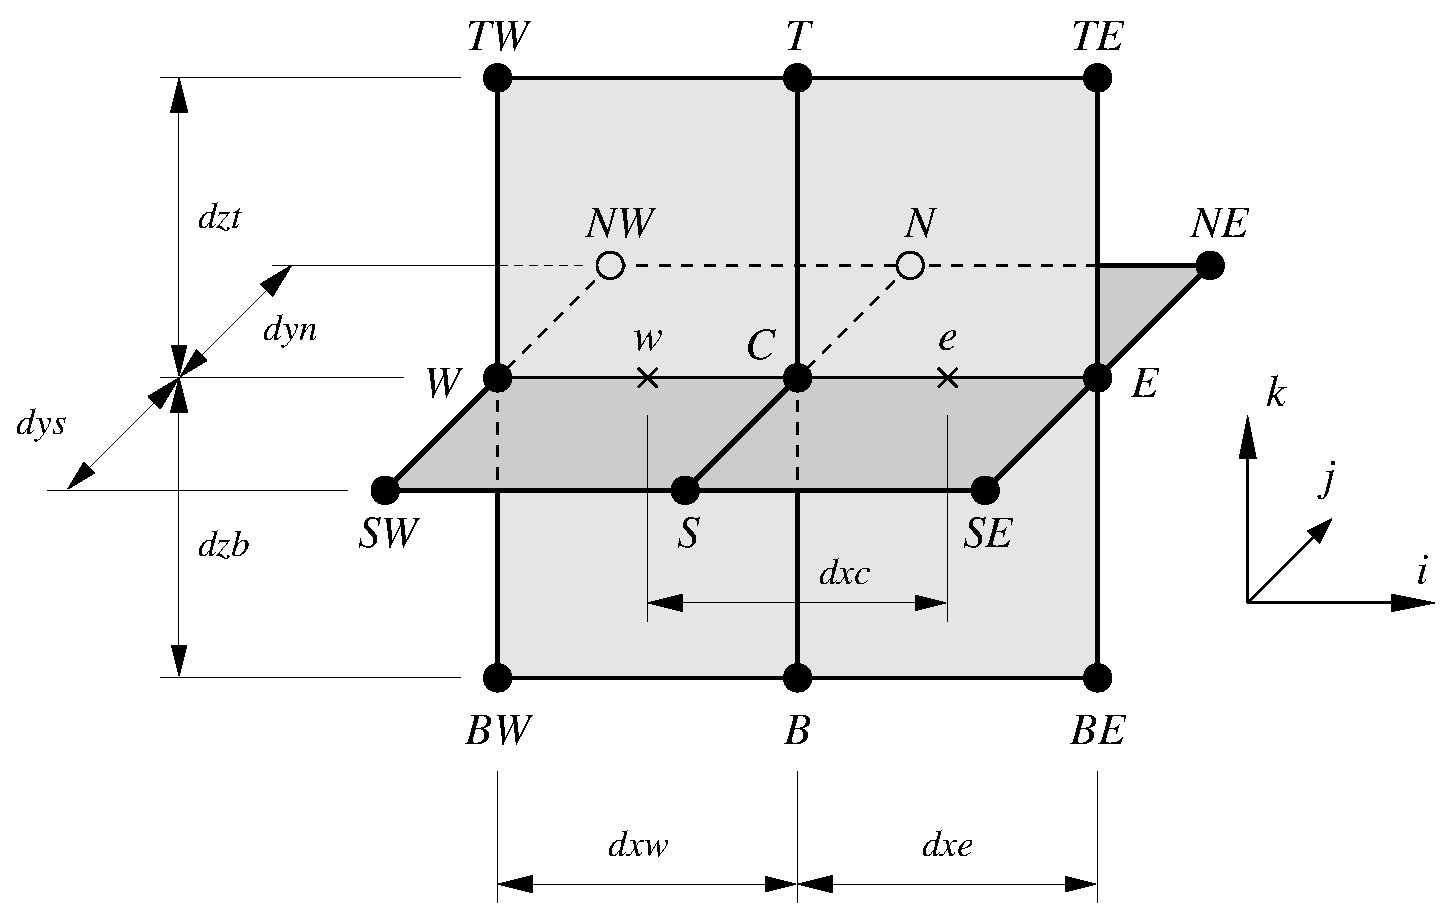
\includegraphics[scale=0.35]{Figures/stencil.eps}}
  \end{picture}
  \caption{Computational stencil.}
  \label{fig:stencil}
\end{figure}
%
\bea
  \frac{\p}{\p x} \left( \frac{\p \phi}{\p x |\nabla \phi|} \right)
  & = &
  \frac{1}{\Delta x_c} 
    \left[
      \left( \frac{\p \phi}{\p x |\nabla \phi|} \right)_e -
      \left( \frac{\p \phi}{\p x |\nabla \phi|} \right)_w
    \right] \nonumber \\
  & = &
  \frac{1}{\Delta x_c} 
    \left(
      \frac{\phi_E-\phi_C}{\Delta x_e |\nabla \phi|_e}  -
      \frac{\phi_C-\phi_W}{\Delta x_w |\nabla \phi|_w} 
    \right) 
\eea
%
Here, $|\nabla \phi|_e$ is evaluated as following:
%
\bea
  |\nabla \phi|_e & = &  \left[ \left(
                          \frac{\phi_E-\phi_C}{\Delta x_e} 
                        \right)^2 \right. \nonumber \\
                  & + & \; \; \, \left( 
                          \frac{\phi_{NE}+\phi_N-\phi_{SE}-\phi_S}
                               {2 (\Delta y_n+\Delta y_s)} 
                        \right)^2 \nonumber \\
                  & + & \; \; \, \left. \left( 
                          \frac{\phi_{TE}+\phi_T-\phi_{BE}-\phi_B}
                               {2 (\Delta z_t+\Delta z_b)} 
                        \right)^2 \right]^{1/2} 
\eea
%
and $|\nabla \phi|_w$ as:
%
\bea
  |\nabla \phi|_w & = &  \left[ \left(
                          \frac{\phi_C-\phi_W}{\Delta x_w} 
                        \right)^2 \right. \nonumber \\
                  & + & \; \; \, \left( 
                          \frac{\phi_{NW}+\phi_N-\phi_{SW}-\phi_S}
                               {2 (\Delta y_n+\Delta y_s)} 
                        \right)^2 \nonumber \\
                  & + & \; \; \, \left. \left( 
                          \frac{\phi_{TW}+\phi_T-\phi_{BW}-\phi_B}
                               {2 (\Delta z_t+\Delta z_b)} 
                        \right)^2 \right]^{1/2} 
\eea
%
Note that, if the numerical grid was uniform, i.e.\ we set:
$ \Delta x_c = \Delta x_w = \Delta x_e = \Delta y_s = \Delta y_n = \Delta z_b = \Delta z_t = \Delta x$,
$|\nabla \phi|_e$ would be evaluated as:
%
\bea
  |\nabla \phi|_e & = &  \frac{1}{\Delta x}
                        \left[ 
                          (\phi_E-\phi_C)^2 
                        \right. \nonumber \\
                  & + & \; \; \; \; \; \; \; \; 
                          (\phi_{NE}+\phi_N-\phi_{SE}-\phi_S)^2 / 16
                        \nonumber \\
                  & + & \; \; \; \; \; \; \; \; \left. 
                          (\phi_{TE}+\phi_T-\phi_{BE}-\phi_B)^2 / 16
                        \right]^{1/2} 
\eea
%
which is the form used by Sun and Beckermann.

%=======================%
%                       %
%  Governing Equations  %
%                       %
%=======================%
\section{Governing Equations}

\be
  \frac{\p \phi}{\p t} + a |\nabla \phi| + {\bf u}_e \cdot \nabla \phi 
= b \kappa |\nabla \phi|
\ee

\be
  \frac{\p \phi}{\p t} + a |\nabla \phi| + {\bf u}_e \cdot \nabla \phi 
= b \left[ \frac{\nabla^2 \phi}{|\nabla \phi|}
          - \frac{(\nabla \phi \cdot \nabla) |\nabla \phi|}{|\nabla \phi|^2} \right]
    |\nabla \phi|
\ee

\be
  \frac{\p \phi}{\p t} + a |\nabla \phi| + {\bf u}_e \cdot \nabla \phi 
= b \underbrace{ \left[ 
     \nabla^2 \phi - \frac{(\nabla \phi \cdot \nabla) |\nabla \phi|}{|\nabla \phi|} 
    \right] }_{\kappa |\nabla \phi|}
\ee
%
We also introduce, without a proof:
%
\be
  |\nabla \phi| = -\frac{\p \phi}{\p n}
\ee
%
\be
  \frac{(\nabla \phi \cdot \nabla) |\nabla \phi|}{|\nabla \phi|} = \frac{\p^2 \phi}{\p n^2}
\ee
%
\be
  \frac{\p \phi}{\p t} - a \frac{\p \phi}{\p n} + {\bf u}_e \cdot \nabla \phi 
= b \underbrace{ \left[ 
     \nabla^2 \phi - \frac{\p^2 \phi}{\p n^2}
    \right] }_{\kappa |\nabla \phi|}.
\ee
%
For no-curvature driven flows, we subtract the term $\kappa |\nabla \phi|$:
%
\be
  \frac{\p \phi}{\p t} - a \frac{\p \phi}{\p n} + {\bf u}_e \cdot \nabla \phi 
= b \left[ 
     \nabla^2 \phi - \frac{\p^2 \phi}{\p n^2}
     - \kappa |\nabla \phi|
    \right],
\ee
%
or, in the form discretized in the system:
%
\framed{\be
  \frac{\p \phi}{\p t} - a \frac{\p \phi}{\p n} + {\bf u}_e \cdot \nabla \phi 
= b \left[ 
     \nabla^2 \phi - \frac{\p^2 \phi}{\p n^2}
     - |\nabla \phi| \nabla \left( \frac{\nabla \phi}{|\nabla \phi|} \right)
    \right].
\ee}
%
The terms $\frac{\p \phi}{\p n}$ and $\frac{\p^2 \phi}{\p n^2}$ should be
discretized using Eqs.~\ref{eq:first_derivation_new} 
and~\ref{eq:second_derivation_new}.


\end{document}             % End of document. 
  
%%%%%%%%%%%%%%%%%%%%%%%%%%%%%%%%%%%%%%%%%%%%%%%%%%%%%%%%%%%%%%%%%%%%%%%%%%%%%%%%
% '$Id: phasefield.tex,v 1.8 2011/05/30 11:50:23 niceno Exp $'/
%%%%%%%%%%%%%%%%%%%%%%%%%%%%%%%%%%%%%%%%%%%%%%%%%%%%%%%%%%%%%%%%%%%%%%%%%%%%%%%%
